\chapter{Background and Motivation}
\label{background}
\quad \textit{Parallel computing} and \textit{software parallelization} are vast, overlapping, and complimentary computer science areas with a rich history dating back to the 1950s. With advances in the semiconductor industry, the topics have left the niche of high-end scientific supercomputers and spread to a much wider area spanning across all consumer electronic devices and have become of major importance.\newline\null
% Parallel computing and software parallelization are vast, complementary and overlapping areas omnipresent across the whole spectrum of hardware. The topics of major importance.
\quad Nowadays, parallelism is pervasive. Parallel hardware is omnipresent across the whole wide spectrum of various computing systems. To exploit all available hardware capabilities software has to be parallel as well. And thus, every computer scientist and software developer would benefit from having an insight into the area. Nonetheless, the topics are extremely complex, require a serious time investment and a great deal of knowledge in various subdomains. It is not realistic to expect an average programmer to possess such deep expertise. For that reason, we propose a solution aimed at alleviating the challenging task of manual software parallelization. Our solution consists of two components. We describe them in Chapters \ref{assistant} and \ref{frameworks}.\newline\null
% Background chapter as the point of basic material accumulation. Based on LLNL tutorials!
\quad In this chapter, we stress the importance of software parallelization, highlight its challenges, describe the parallel software engineering process, and finally lay the ground for our proposed solutions from Chapters \ref{assistant} and \ref{frameworks}. \textbf{The major ideas leading towards the solutions from Chapters \ref{assistant} and \ref{frameworks} are highlighted with boldface text.} We express our special gratitude to Lawrence Livermore National Laboratory (LLNL) \cite{llnl_computing} for their great parallel computing tutorials. We heavily relied on those to prepare the background material.\newline\null
% The story line:
%
% Parallel computing importance
% Challenges of software parallelization:
%     automatic
%     manual
%     machine learning based
%     data-centric parallelization problem
% 
%
\quad The background chapter is structured as follows. Section \ref{background_importance} stresses the importance of parallel computing and software parallelization in the modern world. There are numerous software parallelization methods and techniques, but all of them run into specific challenges and problems. Section \ref{background_challenges} highlights the major problems of various software parallelisation methods. First, it presents the challenges of manual and then automatic software parallelization techniques. There have been various experiments and works employing machine learning (ML) based methods \cite{ml-oboyle} for the task of software parallelization. These challenges form the ground for our program loop parallelization assistant solution \cite{assistant-aiseps} to grow. We describe our solution in Chapter \ref{assistant}. Then, in Section \ref{background_dcp} we discuss the problem of data structure choice and how it affects software parallelization. Unfortunately, there are no universal automatic solutions to this problem at the moment. Data structures are often inseparable from the algorithms they support. Our computational frameworks build on that fact by defining the blend of data structures and algorithms. We propose our solution to the problem in Chapter \ref{frameworks}. Furthermore, modern software design and engineering tasks are extremely rich and complex topics. That is true of parallel software engineering as well of course. In Sections \ref{background_programming_paradigms} and \ref{background_oop_design} we talk about imperative, functional and object-oriented programming paradigms, as well as various OOP software design patterns. Our computational frameworks take the best from these principles and alleviate

\section{The importance of parallel computing}
\label{background_importance}
\quad Parallelism is pervasive and the future of computing is parallel. Many factors stress the importance of parallelism in the modern computing world.
\begin{description}[style=unboxed,leftmargin=0cm]
\itemsep0em
\item[Abundance of natural parallelism] The field of High-Performance Computing (HPC) has traditionally been concerned with scientific modeling and simulation of various natural phenomena (climate change, fluid flows, etc.). Physical systems consist of numerous, often independent parts. Moreover, these problems are often expressed through common parallelizable mathematical models: parallel Gauss \cite{SHANG20091369} and Conjugate Gradient methods \cite{10.1007/978-3-642-14390-8_14}, \cite{HELFENSTEIN20123584} for solving linear equation systems, parallel matrix inversion \cite{SHARMA201331}, parallelizable optimizations for specific cases (like sparse matrices \cite{CHEN201849}, \cite{DEVECI201833}), etc. When we compile a highly parallel algorithm to a serial sequence of CPU instructions or process a huge dataset with independent parts sequentially, we artificially constrain a vastly parallel computation to a serial one.
\item[Semiconductor technology advances and power limits] With advances in transistor density, it became feasible to design more complicated CPUs. Initially, the trend went towards more complex microarchitecture with deeper pipelines, but running into power limits the industry design shifted towards multi-core CPUs and multiprocessor systems. To exploit such systems fully, software must mirror the trend and become parallel as well.
\item[Domain inherent parallelism and specialized computations] The areas like computer graphics for instance have a lot of problems that can be processed in a Single Instruction Multiple Data (SIMD) fashion. That naturally led to the emergence of specialized co-processors like GPUs making hardware systems more complex and heterogeneous \cite{cpu-heterogenuity}.
\end{description}
\quad To fully exploit all capabilities provided by modern high-performance computing systems, software has to be mapped onto the parallel hardware i.e parallelized.

\section{Challenges in software parallelization}
\label{background_challenges}
\quad The problem of software parallelization is extremely complex and multi-faceted. There are various approaches to the problem, but all of them have their pros and cons. Although the process of software parallelization has characteristically been a very \textit{manual} task, which is time-consuming and error-prone, there are also \textit{automatic} and \textit{machine learning based} techniques. In this section, we highlight the inherent problems of all these approaches. The solution we propose grows on these challenges.
\subsection{Manual parallelization challenges}
\label{background_challenges_manual}
\quad Parallel software development has characteristically been a very manual process. Like any software development process, it consists of several stages. The major problems are described below.
\begin{description}[style=unboxed,leftmargin=0cm]
\itemsep0em
\item[Problem understanding and partitioning] As the best software engineering practices dictate, before diving into software development one needs to thoroughly understand the problem and decide on the requirements and restrictions the final piece of software must meet. The whole algorithm and software architecture might change with the decision of developing a parallel software version instead of a serial one. If one starts from an already implemented serial software version, the parallelization might be even more difficult to do. Source code comprehension is a hard task. The algorithm chosen for a serial version might be completely unsuitable for a parallel implementation. The problem must be partitioned into relatively independent chunks of work to be processed in parallel. The partitioning can be done in multiple ways and a programmer needs to choose one (data set decomposition, functional decomposition, or a hybrid of the two).
\item[Communications and synchronization] Very often the parts of the problem are not completely independent and require an exchange of information. Designing the way that exchange is going to work is a complex task. Almost always communication results in overhead. Sending the data over a congested network or waiting on a synchronization barrier slows the program down. The slowdown might even diminish all performance benefits obtained from parallelization.
\item[Implementation and data dependencies] When the problem partitioning is done, all communication and synchronization points are determined and the high level parallel algorithm is designed, a programmer might start the actual implementation. Here a programmer will run into other types of problems. Consider two functionally equivalent code samples below.\newline\null
\begin{minipage}[t]{0.50\linewidth}
\begin{lstlisting}[caption={\raggedright Non-parallelizable loop with planted loop-carried data dependence.},label={lst:code_sample_data_dependence},language=C]
for (int i=1; i<n; i++) {
  a[i]=a[i-1]+1;
}
\end{lstlisting}
\end{minipage}
\begin{minipage}[t]{0.50\linewidth}
\begin{lstlisting}[caption={\raggedright Parallelizable loop free of any data dependencies.}, label={lst:code_sample_no_data_dependence},language=C]
for (int i=0; i<n; i++) {
  a[i]=a[0]+i;
}
\end{lstlisting}
\end{minipage}

The actual shape of the code can break parallelization by introducing fake (not required by the algorithm) dependencies.
\item[Performance analysis and tuning] One needs to know where the program's hotspots are. Hotspots are the places where most of the real work is done. The majority of programs spend most of the CPU time in a few places. The task of a programmer is to find those places and concentrate all parallelization and optimization efforts there. Finding hotspots might be difficult before the programmer has the whole program implemented. Modern hardware architectures have a multi-level memory hierarchy, memory data prefetchers, TLBs, out-of-order execution, etc. It might be surprising how the actual program execution performance differs from the one inferred from the algorithm. Profilers and other analysis tools can help here \cite{perf-tool}.
\end{description}
\quad Finally, all the above challenges are interrelated and very often depend on each other. The parallel software development process can go iteratively with numerous dead ends and redesign efforts. With a long research history into the topic, all these problems are still actual to this day.
\subsection{Limitations of automatic techniques}
\label{background_challenges_automatic}
\quad Given the difficulty of manual software parallelization, there have been numerous ongoing efforts into various automatic parallelization tools. The vast amount of legacy sequential software developed over the last few decades further exacerbates the need. Automatic parallelization refers to converting sequential code into multi-threaded and/or vectorized code in order to use multiple processors simultaneously in a shared-memory multiprocessor (SMP) machine.\newline\null
\quad There are various tools available to a programmer for automating the task of software parallelization. We present an overview of the field in the Section \ref{related_work_autopar}. Parallelizing compilers are the most widely used nowadays. Automatic parallelization tools can be classified into two types:
\begin{description}[style=unboxed,leftmargin=0cm,noitemsep]
\itemsep0em
\item[Fully Automatic] The compiler analyzes the source code and identifies opportunities for parallelization. The analysis includes identifying inhibitors to parallelism and possibly a cost weighting on whether or not the parallelization would improve performance \cite{Kennedy:2001:OCM:502981}. Loops are the most frequent target for automatic parallelization \cite{Bacon:1994:CTH:197405.197406}.
\item[Programmer Directed] Using compiler directives or possibly compiler flags, a programmer explicitly tells the compiler how to parallelize the code. These directives and flags may be also used in conjunction with some degree of automatic parallelization. The most common compiler-generated parallelization is done using on-node shared memory and threads (such as OpenMP \cite{Dagum:1998:OIA:615255.615542}).
\end{description}
\quad If one starts with an existing serial code and has the time or budget constraints, then automatic parallelization may be the answer. However, several important caveats apply to automatic parallelization.
\begin{description}[style=unboxed,leftmargin=0cm]
\itemsep0em
\item[Performance] Performance may degrade.
\item[Limitations] Limited to a subset (mostly loops) of code.
\item[Effectiveness] May not parallelize the code, i.e. it may be "over-conservative" or the code is too complex.
\end{description}
\quad To clearly illustrate the problems an automatic software parallelization faces we conducted several experiments with the suite of NASA Parallel Benchmarks (NPB) \cite{nasa-parallel-benchmarks}. These benchmarks target the performance evaluation of highly parallel supercomputers. Consequently, the suite has a great amount of inherent parallelism and is supposed to be easily parallelizable. NPB benchmarks do not provide the exact implementation, they rather specify what should be computed and how. We used Seoul National University's (SNU) implementation \cite{snu-npb-benchmarks} of NPB benchmarks. SNU NPB implementation comes in two versions: sequential legacy C implementation and the one parallelized with OpenMP pragmas. The main data structure used everywhere in the suite is a simple flat array. Numerous loop nests operate over arrays and compute simple reductions.\newline\null
\quad For these experiments we used a desktop Ubuntu 18.04 machine with installed Intel C/C++ Compiler (ICC) 18.0 and measured the running time of benchmarks with the help of UNIX time() utility. To minimize the errors, we ran experiments several times and took the mean average. The machine has 4 Intel Core i5-6500 CPUs with 3.20 GHz frequency and vectorization support up to AVX2. The RAM is 16Gb.\newline\null
\quad The first experiment we conducted was aimed at assessing the effectiveness of the state-of-the-art automatic parallelization. The experiment is platform agnostic as long as the target supports vector instructions and parallel primitives and can be reproduced on any such platform. We took the Intel C/C++ Compiler (ICC), configured it for the most aggressive parallelization (\textit{-par-threshold0}), i.e parallelize all parallelizable code independent of its potential cost weighted profitability. Also, we configured ICC to do all enabling loop transformations (\textit{-O3} flag) before the actual parallelization (\textit{-parallel} flag) and vectorization (\textit{-vector} flag). In other words, the experiment measures the maximum parallelization coverage the best state-of-the-art compiler can achieve on embarrassingly parallel problems, which still represent the real-world code. Our results show a significant potential for improvement. Among all 1415 SNU NPB loops, 980 are truly parallelizable, but the ICC compiler manages to find only 812 parallelizable cases and misses 168 loops. Table \ref{tab:icc_missed} shows the classification we conducted by manually examining the ICC parallelization reports as well as looking at the source code of the benchmarks. The biggest problems are statically unknown pointers, which might potentially overlap at the running time, as well as other statically unresolvable dependencies. There are some unrecognized reductions as well as loops that can be parallelized with prior array privatization and function inlining.
\begin{table}
  \begin{minipage}{\pagewidth}
  \begin{center}
    \begin{tabu}{M{3.0cm}M{1.0cm}M{3.0cm}M{1.0cm}M{3.0cm}M{1.0cm}}
      \hline
      \rowfont{\bfseries}
      reason & num & reason & num & reason & num\\\hline
      \textbf{unrecognised reduction} & 18 & \textbf{array privatization} & 7 & \textbf{AA conservativeness} & 60\\\hline
      \textbf{unknown iteration number} & 7 & \textbf{static dependencies} & 46 & \textbf{too complex} & 22\\\hline
      \textbf{uninlined calls} & 4 & \textbf{other} & 4 & \textbf{total} & 168\\\hline
    \end{tabu}
  \end{center}
  \end{minipage}
  \caption{Classification of loops missed by Intel Compiler for various reasons.}
  \label{tab:icc_missed}
\end{table}\newline\null
\quad While parallelization coverage is important it is not the primary goal. A parallelized loop might not make a significant contribution to the total running time of the application. We should strive to parallelize those loops, which are on the critical paths and hot spots. And finally, only the running time is the ultimate parallelization performance measure. Given that, we conducted a further experiment. We used the same machine and compiled SNU NPB benchmarks with different sets of ICC automatic parallelization options. Figure \ref{fig:benchmarks_runtime} illustrates the running times of resulting codes. Bars marked as serial (s) show running times of original legacy C sequential versions. Bars marked as omp (o) show running times of an expertly manually parallelized versions. Other bars show running times of versions produced with various combinations of ICC compiler options (vectorize, parallelize or do both), as well as complete cases of parallel OpenMP versions, which have been additionally parallelized and vectorized by the ICC compiler. One can see that the best performance is still attributed to benchmark versions, which have been expertly parallelizad by their developers. Vectorization and parallelization help parallel versions a bit, but not that significantly and the profits can be neglected altogether. When we automatically vectorize serial versions we get a little improvement, but when we try to automatically parallelize them we get striking slowdowns on some benchmarks. Overall, automatic vectorization gives us a tiny 1.1x running time improvement in the geometric mean compared to 1.73x of manual parallelization. And the automatic parallelization results into 0.79x slowdown in the geometric mean across all the benchmarks.\newline\null
\textbf{\quad Our machine learning based loop parallelization assistant \cite{assistant-aiseps} we propose in Chapter \ref{assistant} extends parallelism recognition capabilities of the Intel C/C++ Compiler (ICC) by learning the loop parallelizability property and making predictions regarding it with an acceptable false positives rate. These predictions cover most of the cases missed by ICC. Moreover, our assistant helps to reach the best possible manual expert performance faster by guiding the programmer towards to the most fruitful code segments to parallelize.}
\begin{figure}[ht]
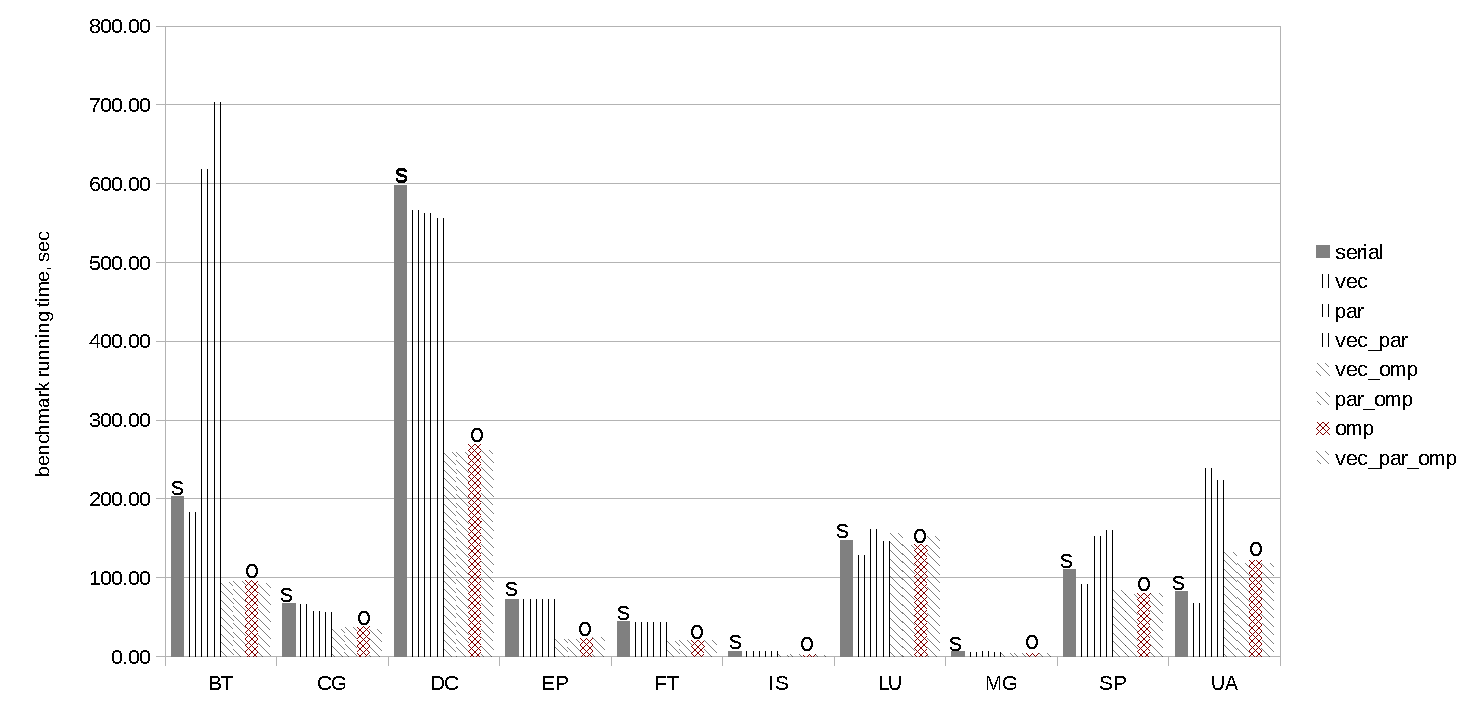
\includegraphics[width=1.0\textwidth]{images/benchmark_runtime.pdf}
\caption{The running time of various NPB benchmarks versions.}
\label{fig:benchmarks_runtime}
\end{figure}
\subsection{Limits of machine learning based methods}
\label{background_challenges_ml}
\quad Correctness is the most important property of the code. Although important, the running time or any other type of code performance characteristic is not always vitally critical. As all machine learning based techniques have always been characterized by their inherent and ineradicable errors \cite{James:2013:ISL:2517747}, the field of compilers and especially the problem of automatic parallelization have never been the primary targets for these methods. Section \ref{related_work_ml} discusses the relevant work in more details. The application of machine learning based methods to the problem of software parallelization has not yet found a widespread practical utility. Mispredictions regarding the code parallelizability can lead to a broken dependency property and thus incorrect program execution. Nonetheless, there have already been works on predicting loop parallelizability, like the approach of Fried \emph{et al.}~\cite{fried_ea:2013:icmla}. Fried \emph{et al.} train a supervised learning algorithm on code hand-annotated with OpenMP parallelization directives to create a loop parallelizability predictor. These directives approximate the parallelization that might be produced by a human expert. Fried \emph{et al.}~focus on the comparative performance of different ML algorithms and studies the predictive performance that can be achieved on the problem and does not produce any practical application.\newline\null
\textbf{\quad In Chapter \ref{assistant} we describe a practical ML-based loop parallelization assistant \cite{assistant-aiseps}. Contrary to Fried \emph{et al.}~\cite{fried_ea:2013:icmla} it uses static source code features. Moreover, we use a richer training set, which is not limited to OpenMP pragmas only, but additionally takes the information from the Intel C/C++ Compiler. While Fried \emph{et al.}~focus on the comparative performance of different ML algorithms and study the possibility to learn loop parallelizability property, we do the same, but
additionally, we contribute a practical assistant capable of
ranking loop candidates in their order of merit.}
\section{Data-Centric Parallelization (DCP) problem}
\label{background_dcp}
\quad The problem of data-centric parallelization (DCP) is the central motivation for the concept of computational frameworks we propose in Chapter \ref{frameworks}. As it has already been stated the problem of software parallelization is multifaceted. There is a vast range of lower level technical issues, which can turn a perfectly parallelizable at a higher level computation into a non-parallelizable implementation. For example, in Section \ref{background_challenges_automatic} we showed that the main reasons of Intel Compiler failures on SNU NPB benchmarks are alias analysis conservativeness, uninlined function calls and statically unresolvable dependencies. These reasons do not close the set of all possible parallel algorithm implementation failures. Listings \ref{lst:array} and \ref{lst:list} clearly illustrate a yet another potential implementation failure.\newline\null
\begin{minipage}[t]{0.5\linewidth}
\begin{lstlisting}[caption={\raggedright Parallelisable loop operating on what is clear to compiler a \textbf{linear array}.},label={lst:array},language=C]
int a[1024];
for (int i=0; i<1024; i++) {
  a[i]=a[i]+1;
}
\end{lstlisting}
\end{minipage}
%
\begin{minipage}[t]{0.5\linewidth}
\begin{lstlisting}[caption={\raggedright Non-parallelisable loop operating on what programmer knows is a \textbf{linked-list}.},label={lst:list},language=C]
struct Node* nptr;
for (p=nptr; p!=NULL; p=p->next) {
  p->value+=1;
}
\end{lstlisting}
\end{minipage}

\quad The above code snippets present two alternative implementations of the same simple and embarrassingly parallel computation. We increment all sequence elements by one. Listing \ref{lst:array} implements the sequence with a regular array linearly laid out in the memory. Listing \ref{lst:list} chooses a linked list as an implementing data structure. While in an array-based implementation the compiler knows all element addresses statically and can generate parallel code in advance in the linked list based implementation element addresses can be resolved only dynamically, which leads to a source code non-parallelizability. Furthermore, compiler does not know what kind of a pointer-based data structure we iterate over.\newline\null
\quad The data-centric parallelization problem is how to automatically recognize what kind of a data structure is used in the code: is it a tree, a linked-list, a directed acyclic graph? The DCP problem is not solved yet. Automatic methods are limited in their recognition capabilities to relatively simple code bases such as libraries of well-known data structures. Automatic transformation is even harder. The most successful methods rely on the dynamic analysis of memory graphs. Static techniques such as shape analysis are undecidable and highly conservative and might not finish in a reasonable time for the real software projects. The section \ref{related_work_dcp} gives a comprehensive literature review on the topic.
\section{Imperative and functional programming}
\label{background_programming_paradigms}
\quad Programming languages can be classified by different \textit{programming paradigms} they support. Among the most general classifications are \textit{imperative} and \textit{declarative} programming languages.\newline\null
\quad Imperative programs are written in a form of instruction sequences, which read and write the \textit{state} of a program. The concept of state is the main characteristic of the imperative programming paradigm. Instruction sequences can be structured in various ways. In \textit{procedural programming} paradigm instructions are grouped inside procedures and functions. In \textit{object-oriented programming (OOP)} paradigm instructions are grouped with the data they operate on inside objects of various types or classes. Programs are built either out of various procedures calling each other and exchanging the data or on the interaction of objects of various types. Imperative programs specify the exact sequence of steps to take in order to compute the final result.\newline\null
\quad Declarative programs do not specify the exact sequence of steps and state updates a program needs to do to get the desired result. Declarative programs declare the properties of the desired result. The properties can be specified as a set of constraints like in \textit{constraint programming} or a set of linear inequalities like in \textit{linear programming}. \textit{Functional} programming is another subtype of declarative programming. In functional programming, the final result is specified as a sequence of stateless function evaluations, which form a tree of expressions. Among the most common constituents are functions like \textit{map}, \textit{reduce}, \textit{fold}, etc. Functions can be passed as arguments and returned from other functions ultimately composing bigger programs.\newline\null
\quad Functional programming is sometimes treated as synonymous with purely functional programming, a subset of functional programming that treats all functions as deterministic mathematical functions, or pure functions. When a pure function is called with some given arguments, it will always return the same result, and cannot be affected by any mutable state or other side effects. This is in contrast with impure procedures, common in imperative programming, which can have side effects (such as modifying the program's state or taking input from a user). Proponents of purely functional programming claim that by restricting side effects, programs can have fewer bugs, be easier to debug and test, and be more suited to formal verification.\newline\null
\quad There are no universally optimal programming paradigms and languages. Some languages are more convenient and suitable for one sort of problem, some languages are better at tackling other problems. For example, functional languages are more convenient in addressing certain domains such as R for statistics and financial analysis. Imperative languages are certainly better for simulations and other state-based scientific computations. For that reason, major languages are often multi-paradigm to cover a potentially larger set of problems. Largely imperative C++ language included support for functional programming with its newer standards starting from C++11.\newline\null
\quad \textbf{There is still an unfilled gap between functional and imperative programming paradigms: some problems contain computations, which are better expressed with standard functional concepts (like \textit{maps}, \textit{folds}, \textit{reductions}, etc.), but at the same time require some state keeping. These problems lie at the boundary of functional and imperative programming. In Chapter \ref{frameworks} we propose an idea of \textit{computational frameworks}, which fills that gap. Moreover, we develop a prototype library \cite{frameworks-repo} with a modern and convenient programmer interface, which takes the best features of both object-oriented and functional paradigms and reflects the core ideas behind the concept of computational frameworks.}
\section{OOP and software design patterns}
\label{background_oop_design}
\subsection{Object-Oriented Programming (OOP)}
\label{background_oop}
\quad \textit{Object-oriented programming (OOP)} is arguably the most widely used programming paradigm nowadays. It is supported by almost all major programming languages. At the very essence, in OOP computer programs are designed by making them out of objects that interact with one another. Object interactions are very close to the human level of reasoning and logic and thus the paradigm fits quite naturally to a human developer.\newline\null
\quad Objects are instances of different types or classes in OOP terminology. Classes are object specifications. They specify the data objects contain (like an integer \textit{age} field for an object of class \textit{Person}) and the methods used to operate on the data. Classes define the public part of objects as well as their internal implementation. Object-oriented (OO) languages provide a rich set of facilities and features to build programs.\newline\null
\quad \textit{Encapsulation} is used for protection against object misuse and unintended outside interference: data and methods concerned with internal workings are declared \textit{private}, while those designed to form an outward appearance are declared \textit{public}. This facilitates code refactoring, for example allowing the author of the class to change how objects of that class represent their data internally without changing any external code. It also eases debugging by better localizing functionality and thus possible bugs.\newline\null
\quad \textit{Dynamic dispatch} is the responsibility of the object, not any external code, to select the procedure to execute in response to a method call, typically by looking up the method at run time in a table associated with the object. This feature allows a programmer to write general code, which works with abstract interface methods and leaves the exact method resolution to be made during the running time of a program.\newline\null
\quad Dynamic dispatch is closely related to the technique of \textit{inheritance}. Inheritance allows classes to be arranged in a hierarchy that represents "is-a-type-of" relationships. Inheritance can be of two types: interface and implementation inheritance. The first one allows a parent class to require its descendants to stick to the same interface. A common interface allows the objects of different classes from the same hierarchy to be operated on by the same type agnostic code. The latter is called a \textit{polymorphism}. The user code can be more concise and abstract. The call of the same method on the parent class or one of its descendants can result in a varying behaviour.\newline\null
\quad Features that are described above do not close the set of all available OOP techniques and mechanisms. These are just the main features we rely on in our project of computational frameworks and are the most important to know.
\subsection{Software design patterns}
\label{background_design}
\quad The presence of all the above features makes OOP languages extremely rich with various facilities. That creates a vast design space for software architects and turns the OOP software design into an art. \textit{Software design patterns} \cite{gang-of-four} are reusable solutions to common design problems in OOP. Design patterns have been well tested and are proven to be the most reliable and elegant solutions for the design problems they target.\newline\null
\quad Design patterns live at an intermediate level between the exact algorithm and a programming paradigm and are language agnostic. Design patterns specify and document solutions to common design problems. These solutions consist of a set of classes, objects, and the ways they interact with one another. It is agreed to classify patterns into 4 distinct categories: creational, structural, behavioral, and concurrency patterns. Here we are going to mention only those patterns, which are the most relevant to our project of computational frameworks.\newline\null
\quad The \textit{command} pattern is a behavioral pattern, where a command object is used to encapsulate all the information needed to perform an action or trigger some event at a later time. The other participants are the receiver, invoker, and client. The central ideas of this design pattern closely mirror the semantics of first-class functions and higher-order functions in functional programming languages. Specifically, the invoker object is a higher-order function of which the command object is a first-class argument.\newline\null
\quad One can see the command pattern used in combination with the \textit{chain of responsibility pattern}, which is a design pattern consisting of a source of command objects and a series of processing objects. Each processing object contains logic that defines the types of command objects that it can handle; the rest are passed to the next processing object in the chain. In a variation of the standard chain of responsibility model, some handlers may act as dispatchers, capable of sending commands out in a variety of directions, forming a \textit{tree of responsibility}. The chain of responsibility pattern promotes the idea of \textit{loose coupling}, where the system consists of multiple components, which know little or nothing about the definitions of other components.\newline\null
\quad Another very relevant pattern is a \textit{template method} pattern. The template method is a method in a superclass, usually an abstract superclass, and defines the skeleton of an operation in terms of a number of high-level steps. These steps are themselves implemented by additional helper methods in the same class as the template method. The helper methods may be either abstract methods, for which case subclasses are required to provide concrete implementations, or hook methods, which have empty bodies in the superclass. Subclasses can (but are not required to) customize the operation by overriding the hook methods. The template method intends to define the overall structure of the operation while allowing subclasses to refine, or redefine certain steps.\newline\null
\quad The \textit{visitor} pattern is a way of separating an algorithm from an object structure on which it operates. A practical result of this separation is the ability to add new operations to existing object structures without modifying the structures. In essence, the visitor allows adding new virtual functions to a family of classes, without modifying the classes. Instead, a visitor class is created that implements all of the appropriate specializations of the virtual function. The visitor takes the instance reference as input and implements the goal through double dispatch.\newline\null
\quad Software design patterns can be more down to the language like the \textit{curiously recurring template pattern (CRTP)}, which is an idiom in C++ where class X derives from a class template instantiation using X itself as template argument.\newline\null
\quad \textit{Software design patterns} specify and document the best practices to solve various commonly reoccurring problems. In the end, it is the experience, mastery, and ingenuity of a programmer which determine the final software design.  
\subsection{Computational frameworks and design patterns}
\label{background_design_frameworks}
\quad When we introduce the concept of computational frameworks, it is very important to mention software design patterns. While not the same, the two concepts have an overlap. Computational frameworks do not specify the exact algorithms and data structures that must be used to implement the task, but like declarative programming rather define the requirements on a higher level computation. For instance, a fractal can be implemented as a tree or as a heap and a fold can be implemented with an array or with a linked list, but the higher-order computational requirements must be met. One can see a similarity to the template method design pattern, which also specifies the main computation and leaves some lower-level steps to be defined by a user. One can see a similarity between the chain of responsibility pattern and the fold computational framework. The latter is also a visitor pattern in its way. While the backbone computation of our frameworks is implemented with a template method pattern, the command pattern is used to specify the user-defined custom part. Computational frameworks also promote the idea of loose coupling by keeping the computational procedure strictly decoupled from the side effects accumulation.\newline\null
\textbf{\quad Computational frameworks embody the best ideas of all relevant software design patterns (template method, command, curiously recurring template pattern, etc.) and can be also considered as such. They relieve a programmer from a complex task of software architecture design by providing ready solutions with all computational, communicational, and data access patterns known and implemented in advance.}
\section{Algorithmic skeletons and Parallel design patterns}
\label{background_skeletons}
\quad An overview paper \cite{skeletons-overview} presents the concepts of \textit{algorithmic skeletons} (or \textit{parallelism patterns}) and \textit{parallel design patterns} and tracks the way how these concepts have permeated the mainstream parallel programming community. We heavily relied on this work to prepare the material below.\newline\null
\quad In the last two decades the general purpose computing industry has made a massive shift towards parallelism. The number of various parallel hardware architectures available on the market has substantially increased. The change is not just quantitative: the number of parallel CPUs and CPU cores has increased, as well as the diversity and heterogeneity of parallel computing systems \cite{welcome-to-the-jungle}. Modern systems feature various accelerators such as GPUs integrated together with possibly networked parallel CPU clusters into rather heterogeneous and complex computing environments.\newline\null
\quad The already difficult task of parallel programming (see Section \ref{background_challenges_manual}) has become even more challenging and the need for adequate programming models and frameworks to ease the job of parallel application programmers has become acute. As hardware architectures become pervasively parallel and grow in their complexity, there is an ongoing effort to address the ease of programmability of the next generation computing systems. Various structured parallel programming models have been proposed to tackle the problem.\newline\null
\quad Analogous to structured sequential programming, where \textit{if-then-else}, \textit{switch statement}, etc. have replaced unstructured goto-based programming style, parallel structured programming models ban certain programming practices. Concurrency can only be expressed and orchestrated through well-established parallel "forms" and structured compositions of those. Structured parallel programming fosters not only more maintainable code, but also makes it more parameterizible and predictable in terms of performance behaviour.\newline\null
\quad Relatively low-level standards like POSIX threads no longer meet all emerged requirements to harness underlying hardware complexity and diversity and at the same time provide a convenient abstraction to application programmers. A number of further "de facto standards" like OpenMP for shared memory architectures, CUDA and OpenCL for GP-GPUs, MPI for distributed systems have been designed and introduced into the industry. Furthermore, the key industry players proposed other higher level frameworks such as IntelTBB or Microsoft PPL. Arguably, these models encompass the key results from an academic research in the area of parallelism patterns.
\begin{description}[style=unboxed,leftmargin=0cm,noitemsep]
\itemsep0em
\item[Algorithmic skeletons or Parallelism Patterns] The algorithmic skeleton (parallelism pattern) concept was introduced into the academia by Murray Cole in his PhD thesis in the late ’80s \cite{mcole-thesis}. Algorithmic skeleton concept is intended to address the difficulty of programming parallel hardware architectures by separating two concerns: expressing application's parallelism through a composition of well-established and well-known primitives or algorithmic skeletons and designing and developing libraries of these primitives on a system programming side. Since the inception of the concept, a number of various algorithmic skeletons have been proposed. Among the most well-known patterns are \textit{map}, \textit{pipeline}, \textit{reduce}, \textit{scan}, \textit{stencil}, \textit{divide and conquer}, \textit{task farm}, etc. More complex patterns can be composed of the basic ones. Algorithmic skeletons are higher than other parallel programming models and thus more human-friendly and portable. More detailed description can be found in the book on structured parallel programming \cite{mccool-patterns}. For example, a \textit{pipeline} algorithmic skeleton can be defined like this:\newline\null
A \textit{pipeline} is a chain of parallel processing entities arranged in a way so the output of each entity is the input to the next one. Suppose the pipeline consists of $n$ stages described by functions $f_{1},...,f_{n}$. Then, for each data $x$ in the input stream, the functions are applied consecutively to produce the final output $f_{n}(...(f_{2}(f_{1}(x))))$. When the stage $f_{j}$ is done processing its input $x_{i}$, it can start to process the next input element $x_{i+1}$ in the data stream. The next stage $f_{j+1}$, in turn, starts processing $f_{j}(x_{i})$ data now in parallel. There are must be no race conditions between stages.\newline\null
\quad The above description presents a very general high-level specification that frames a parallel computation and leaves some space for creating various versions of the definition. An example of a more constraining definition can be found in the work \cite{skeletons-static} (see Section \ref{related_work_as_and_pp}), which requires functions $f_{1},...,f_{n}$ to be pure, i.e have no side-effects. Though, the violation of this requirement does not break pipeline parallelizability, as long as there are no race conditions between the stages.
\item[Parallel design patterns] The concept of software design patterns (see Section \ref{background_oop_design}) has migrated to the world of parallel programming in '00s. Design pattern is a "recipe", that addresses some specific computational scenario. This recipe describes a problem together with the best known solution. Parallel design patterns are described along the space of 4 dimensions: finding concurrency (i.e what parallelism can we exploit?), algorithm design (finding suitable algorithms), implementation structures and execution mechanisms (multi core CPUs, vector instructions, etc.). The table \ref{tab:pipeline_design_pattern} below illustrates an example of \textit{pipeline} parallel design pattern.
\begin{table*}[!ht]{\linewidth}
  \tabulinesep=2pt
  \begin{minipage}{\linewidth}
  \begin{center}
    \begin{tabu}{M{3cm}M{11.0cm}}
      \hline
      \rowfont{\bfseries}
      Name & Pipeline\\\hline
      Problem & Computation is organized in stages, over a large number of independent data sets\\
      Examples & Assembly line, CPU instruction fetch/decode/execute cycle, video frame processing with multiple filters, etc.\\
      Features & Parallel stage computation, input/output ordering, etc.\\
      Implementation & Set up a chain of parallel activities, each one processing a stage, receiving input data from previous stage and delivering results to next stage through proper
      single-producer single-consumer message queues.\\
      Sample implementation & A sketch of MPI-based code computing a pipeline\\\hline
      \end{tabu}
  \end{center}
  \caption{Sketch of sample pipeline parallel pattern specification (the whole pattern may easily take tens of pages to be
  properly described \cite{mccool-patterns}).}
  \label{tab:pipeline_design_pattern}
  \end{minipage}
\end{table*}%
\end{description}
\quad Algorithmic skeletons and parallel design patterns themselves are largely well-established and are not at the cutting edge of the research effort. At the same time the fifty years of parallel programming has generated a substantial amount of parallel legacy code using lower-level, more hardware-specific and hence less portable, less maintainable code. There is a range of ongoing research efforts to automatically identify various parallelism patterns in a legacy code and substitute them with their rejuvenated modern counterparts. Unfortunately, refactoring tools are still premature and are not fully adopted by development centers yet. In fact, most of them are human-supervised, where a developer is responsible either for approving or doing the final manual transformation of the code. Although these tools relieve the burden of the source-to-source transformation, this process still remains semi-automatic. The Section \ref{related_work_as_and_pp} provides a literature review on the subject.\newline\null
\textbf{\quad Parallel design patterns specify computations on a very high algorithmic implementation-agnostic level, leaving the whole software design and implementation to an application programmer. Algorithmic skeletons implement low-level system side part of parallelization under the hood, alleviating the task for an application programmer. Computational frameworks go further by narrowing their target application to scientific state based simulations accumulating side effects. While algorithmic skeletons or parallelism patterns stress an algorithmic component of the computation, computational frameworks contain an underlying data structure that might accumulate computation's side effects.}
